\documentclass{standalone}
\usepackage{tikz}
\usepackage{ctex,siunitx}
\setCJKmainfont{Noto Serif CJK SC}
\usepackage{tkz-euclide}
\usepackage{amsmath}
\usepackage{wasysym}
\usetikzlibrary{patterns, calc}
\usetikzlibrary {decorations.pathmorphing, decorations.pathreplacing, decorations.shapes,}
\begin{document}
\small
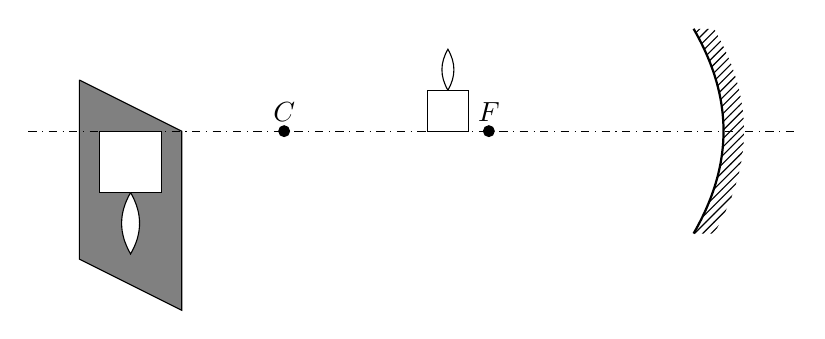
\begin{tikzpicture}[>=latex,scale=1.3]
  \fill [pattern=north east lines] (2,-1)--(2.2,-1) to [bend left=-30] (2.2,1) --(2,1) to [bend left=30](2,-1);
  \draw [thick](2,1) to [bend left=30] (2,-1);
  \node at (0,0)[above]{$F$}; \draw [fill=black] (0,0) circle(1.5pt);
  \node at (-2,0)[above]{$C$}; \draw [fill=black] (-2,0) circle(1.5pt);
  \draw (-.6,0) rectangle (-.2,.4); \draw (-.4, .4) to [bend left=-30](-.4, .8)to [bend left=-30] (-.4,.4) ;
  \draw [fill=gray] (-4, .5)--(-4,-1.25)--(-3, -1.75)--(-3, 0)--(-4, .5);
  \draw [fill=white](-4+.2,0) rectangle (-4+.8,-.6); 
  \draw [fill=white] (-3.5, -.6) to [bend left=-30](-3.5,-1.2)to [bend left=-30] (-3.5, -.6) ;
  \draw[dashdotted] (-4.5,0)--(3,0);
\end{tikzpicture}
\end{document}